\input{preambule-sacha-utf8.ltx}

\usepackage{parcolumns}

        \title {Démonstrations de terminale S - Tronc commun \\
                Lycée International}

        \author{Sacha Dhénin}
        
\usepackage{amsthm}

\usepackage{tikzsymbols}

\begin{document}

%\iffalse

\pgfmathdeclarefunction{gauss}{2}{%
  \pgfmathparse{1/(#2*sqrt(2*pi))*exp(-((\x-#1)^2)/(2*#2^2))}%
}

%\maketitle
\newpage
%\thispagestyle{empty}

%\fi

% POUR LES FIGURES : 
%\def\myscale{.75} % par défaut 
%\newcommand{\myfigure}[2]{  % entrée : echelle, fichier figure
%\def\myscale{#1}\begin{center}\footnotesize{#2}\end{center}}
%\newcommand{\E}{(-4,-1) rectangle (4,4)}
%\newcommand{\A}{(0,0) ++(135:2) circle (1.9)}
%\newcommand{\B}{(0,0) ++(45:2) circle (1.9)}
%\definecolor{myred}{rgb}{0,0,0}
%\definecolor{myorange}{rgb}{0,0,0}

\thispagestyle{empty}

%\setcounter{tocdepth}{4}
%\tableofcontents

%\newpage 

%Remplacer tous les $\varnothing$ par $\emptyset$.

\newpage

\vspace*{-2cm}

\section*{Étude graphique des trinômes du seconde degré}

\subsection*{Premier cas}

Soit $f$ la fonction définie par $f(x) = ax^2 + bx + c$. \\

\definecolor{uuuuuu}{rgb}{0.266666666667,0.266666666667,0.266666666667}
\definecolor{qqffqq}{rgb}{0.,1.,0.}
\definecolor{qqqqtt}{rgb}{0.,0.,0.2}
\definecolor{ffqqqq}{rgb}{1.,0.,0.}
\definecolor{cqcqcq}{rgb}{0.752941176471,0.752941176471,0.752941176471}
\begin{tikzpicture}[line cap=round,line join=round,>=triangle 45,x=1.0cm,y=1.0cm]
\draw [color=cqcqcq,dash pattern=on 2pt off 2pt, xstep=1.0cm,ystep=1.0cm] (-6.92159911725,-5.45164726141) grid (10.1615473692,8.55742232498);
\draw[->,color=black] (-6.92159911725,0.) -- (10.1615473692,0.);
\foreach \x in {-6,-5,-4,-3,-2,-1,1,2,3,4,5,6,7,8,9,10}
\draw[shift={(\x,0)},color=black] (0pt,2pt) -- (0pt,-2pt) node[below] {\footnotesize $\x$};
\draw[->,color=black] (0.,-5.45159911725) -- (0.,8.55742232498);
\foreach \y in {-5,-4,-3,-2,-1,1,2,3,4,5,6,7,8}
\draw[shift={(0,\y)},color=black] (2pt,0pt) -- (-2pt,0pt) node[left] {\footnotesize $\y$};
\draw[color=black] (0pt,-10pt) node[right] {\footnotesize $0$};
\clip(-5.45159911725,-4.45164726141) rectangle (10.1615473692,8.55742232498);
\draw [samples=50,rotate around={0.:(1.,-4.)},xshift=1.cm,yshift=-4.cm,color=ffqqqq,domain=-6.0:6.0)] plot (\x,{(\x)^2/2/0.5});
\draw [color=qqffqq,domain=-6.92159911725:10.1615473692] plot(\x,{(--5.-0.*\x)/1.});
\draw (-5.5,7.80555405587) node[anchor=north west] {$y = ax^2 + bx + c$};
\draw (6.88916244125,4.9527245971) node[anchor=north west] {$y = 5$};
\begin{scriptsize}
%\draw[color=ffqqqq] (0.387259870801,-2.8429988717) node {$c$};
\draw [fill=qqqqtt] (1.,-4.) circle (1.5pt);
\draw[color=qqqqtt] (1.12164283132,-4.25223491806) ; %  node {$S$};
%\draw[color=qqffqq] (-6.78171664858,4.86802221378) node {$a$};
\draw [fill=uuuuuu] (-2.,5.) circle (1.5pt);
\draw [fill=uuuuuu] (4.,5.) circle (1.5pt);
\end{scriptsize}
\end{tikzpicture}

\medskip 

\setbox1=\vbox{\hsize=15mm\begin{center} \dChangey[3]{2}\\ {\it Think positive}\end{center}}

\setbox2=\hbox{$\left\lbrace \begin{array}{lr}
x_1 = & -1 \\
x_2 = & 3
\end{array} \right.$}
\begin{enumerate}
\item Que vaut $a$ ?
\item Que vaut $c$ ? 
\item Que vaut $\alpha$ ? 
\item Que vaut $\beta$ ?
\item Quelles sont les racines ? 
\setlength{\fboxrule}{2pt} 
\item Quelles sont les solutions de {$f(x)\leqslant 0 $} ? 
\item Quelles sont les solutions de  {$f(x) > 5 $} ?  
\end{enumerate}

\newpage

\subsection*{Deuxième cas}

Soit $f$ la fonction définie par $f(x) = ax^2 + bx + c$. \\

\definecolor{uuuuuu}{rgb}{0.266666666667,0.266666666667,0.266666666667}
\definecolor{qqffqq}{rgb}{0.,1.,0.}
\definecolor{qqqqtt}{rgb}{0.,0.,0.2}
\definecolor{ffqqqq}{rgb}{1.,0.,0.}
\definecolor{cqcqcq}{rgb}{0.752941176471,0.752941176471,0.752941176471}
\begin{tikzpicture}[line cap=round,line join=round,>=triangle 45,x=1.0cm,y=1.0cm]
\draw [color=cqcqcq,dash pattern=on 2pt off 2pt, xstep=1.0cm,ystep=1.0cm] (-6.8691431915,-8.00116490393) grid (10.2140032949,5.00790468245);
\draw[->,color=black] (-6.8691431915,0.) -- (10.2140032949,0.);
\foreach \x in {-6,-5,-4,-3,-2,-1,1,2,3,4,5,6,7,8,9,10}
\draw[shift={(\x,0)},color=black] (0pt,2pt) -- (0pt,-2pt) node[below] {\footnotesize $\x$};
\draw[->,color=black] (0.,-8) -- (0.,5.00790468245);
\foreach \y in {-7,-6,-5,-4,-3,-2,-1,1,2,3,4}
\draw[shift={(0,\y)},color=black] (2pt,0pt) -- (-2pt,0pt) node[left] {\footnotesize $\y$};
\draw[color=black] (0pt,-10pt) node[right] {\footnotesize $0$};
\clip(-6.8691431915,-8.00116490393) rectangle (10.2140032949,5.00790468245);
\draw [samples=50,rotate around={-180.:(1.,4.)},xshift=1.cm,yshift=4.cm,color=ffqqqq,domain=-5.0:5.0)] plot (\x,{(\x)^2/2/0.5});
\draw [color=qqffqq,domain=-6.8691431915:10.2140032949] plot(\x,{(-5.-0.*\x)/1.});
\draw (-5.81353838418,-7.17935540049) node[anchor=north west] {$y = ax^2 + bx + c$};
\draw (5.98255861763,-5.01117713609) node[anchor=north west] {$y = -5$};
\begin{scriptsize}
\draw [fill=qqqqtt] (1.,4.) circle (1.5pt);
\draw[color=qqqqtt] (1.12164283132,4.23855110476)  ; % node {$S$};
\draw [fill=uuuuuu] (4.,-5.) circle (1.5pt);
\draw [fill=uuuuuu] (-2.,-5.) circle (1.5pt);
\end{scriptsize}
\end{tikzpicture}


\medskip 

\setbox1=\vbox{\hsize=15mm\begin{center} \dChangey[3]{-2}\end{center}}

\setbox2=\hbox{$\left\lbrace \begin{array}{lr}
x_1 = & -1 \\
x_2 = & 3
\end{array} \right.$}

\setbox3=\vbox{\hsize=75mm Le sommet $\mathcal{S}$ a pour coordonnées $(1,4)$,\\donc $\alpha = 1$ et $\beta :4$}

\setbox4=\vbox{\hsize=75mm On a $\left\lbrace \begin{array}{l}
f(-1) = 0 \\
f(3) = 0 
\end{array} \right.$, donc $\left\lbrace \begin{array}{l}
x_1 = -1 \\
x_2 = 3 
\end{array} \right.$}

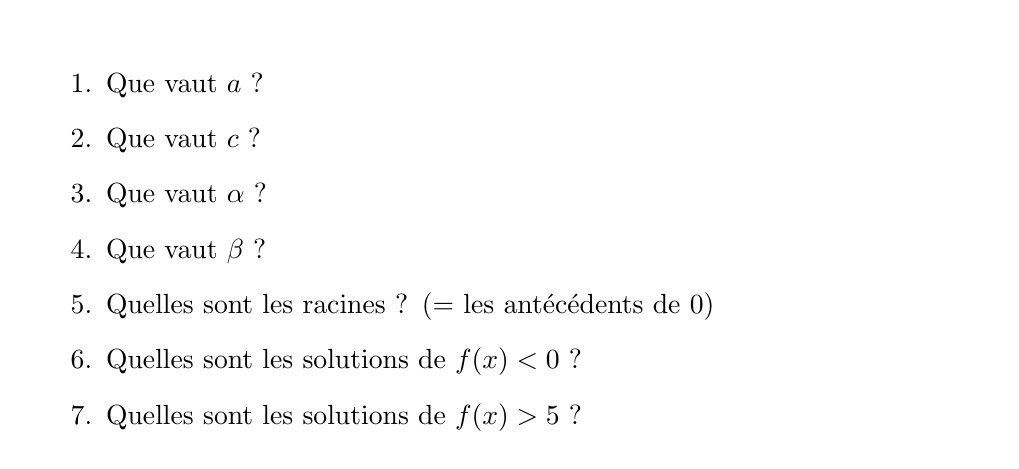
\begin{tikzpicture}[decoration=brace] 
% \draw [color=gray!75,dash pattern=on 2pt off 2pt, xstep=1.0cm,ystep=1.0cm] (0,0) grid (5,5);
 \node[text width=12cm] (box)
{ \begin{enumerate}
\item Que vaut $a$ ? 
\item Que vaut $c$ ? 
\item Que vaut $\alpha$ ? 
\item Que vaut $\beta$ ?  
\item Quelles sont les racines ? 
(= les antécédents de 0)

\setlength{\fboxrule}{2pt} 
\item Quelles sont les solutions de {$f(x) <  0 $} ?  
                          
\item Quelles sont les solutions de  {$f(x) > 5 $} ?  
 
\end{enumerate} } ; % Attention au point-virgule 
% 
\end{tikzpicture}
\end{document}